\documentclass{article}
\usepackage[utf8]{inputenc}
\usepackage[english,serbian]{babel}
\usepackage{graphicx}
\usepackage{amsmath,amssymb}
\usepackage{siunitx}
\usepackage{float}
\usepackage[utf8]{inputenc}
\usepackage[unicode]{hyperref}
\usepackage[lofdepth,lotdepth]{subfig}

\title{Lokalizacija izvora svetlosti}
\author{Petar Marković i Luka Simić}
\date{Jun 2018, IS Petnica}

\begin{document}

\maketitle

\section{Uvod}
    Cilj vežbe je određivanje lokacije objekta (sijalice) pomoću fotootpornika na tabli veličine $\SI{1}{\meter} \times \SI{1}{\meter}$.
    fotootpornik je elektronska komponenta koja menja svoju otpornost u zavisnosti od detektovane količine svetlosti. Otpornost fotootpornika je obrnuto proporcionalna količini prisutne svetlosti.
    % Objasni kako radi fotootpornik
    % Dodaj sliku fotootpornika
    Da bi se iz fotootpornika dobila informacija o jačini svetlosti, fotootpornik se mora povezati na naponski razdelnik. Naponski razdelnik je elektronsko kolo u kom odnos izlaznog napona ($V_{out}$) i ulaznog napona ($V_{in}$) zavisi od odnosa dva otpornika u kolu ($R_1$ i $R_2$) na takav način da:
    $$V_{out} = \frac{R_2}{R_1 + R_2} \cdot V_{in}$$
    Pošto je zavisnost izlaznog napona od udaljenosti fotootpornika od izvora svetlosti različita za svaki fotootpornik, svaki fotootpornik je morao da se kalibriše računanjem zavisnosti udaljenosti izvora svetlosti od fotootpornika od udela izlaznog napona u ulaznom naponu, izraženom u rasponu od 0 do 1023, jer ima 10-bitnu rezoluciju.%  je takve brojeve vraćao \textit{EasyPIC} mikrokontrolerov AD konvertor.
    % Objasniti kako radi AD konvertor?
    \begin{figure}[H]
        \centering
        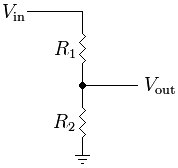
\includegraphics[scale=0.5]{razdelnik.png}
        \caption{Šematski prikaz naponskog razdelnika}
        \label{Razdelnik}
    \end{figure}

\section{Metod rada}
\subsection{Aparatura}
    \begin{itemize}
        \item Tri (odnosno četiri) fotootpornika (sa PFE-brendiranim postoljima)
        \item Protobord
        \item \textit{EasyPIC} model P18F45K22
        \item Tri (odnosno četiri) otpornika od \SI{1}{\kilo\ohm} % Je l' bilo 1kOhm?
    \end{itemize}
    \begin{figure}[H]
        \centering
        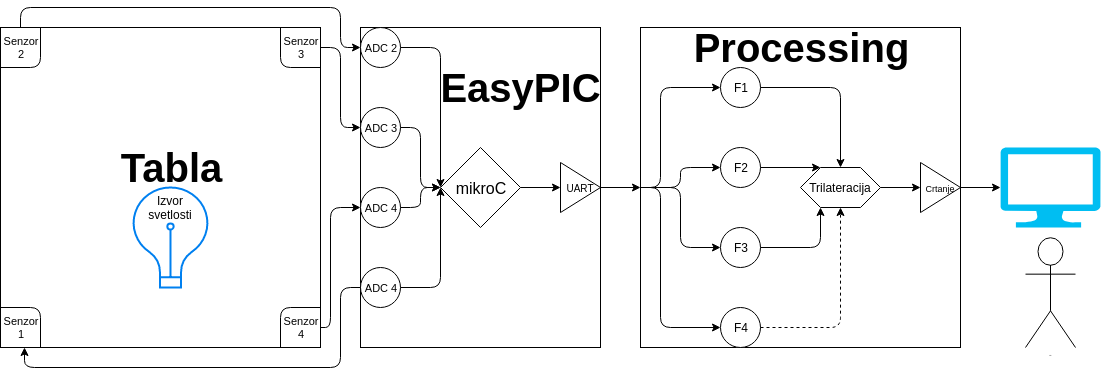
\includegraphics[scale=0.3]{dijagram.png}
        \caption{Dijagram rasporeda aparature i protoka podataka}
        \label{Dijagram}
    \end{figure}

\subsection{Metod}
    Vežba je rađena u potpuno tamnoj prostoriji sa ugašenim svetlima, kako bi očitavanje senzora bilo što tačnije. Prostor za realizaciju vežbe se nalazio na stolu podeljenom na $40\times40$ kvadrata, međusobno udaljenih \SI{2.5}{\cm} u čijim temenima su se nalazile rupice koje su korišćene za lakše merenje.

    Senzori (foto-otpornici na postoljima) koji su bili korišćeni nisu iste otpornosti i kvaliteta, zbog čega je bilo potrebno izvšiti kalibraciju posebno za svaki. Kalibracija je vršena merenjem napona na svakoj tački dijagonale prema kojoj je senzor bio okrenut. Izvršeno je 117 merenja po dijagonali, jer je za svaku od 39 tačaka dijagonale u kojima se merenje moglo izvršiti mereno po tri puta zbog neidealnosti (greške) senzora. Rezultati merenja mogu se videti na slici \ref{Kalibracija}.

    \begin{figure}[H]
        \centering
        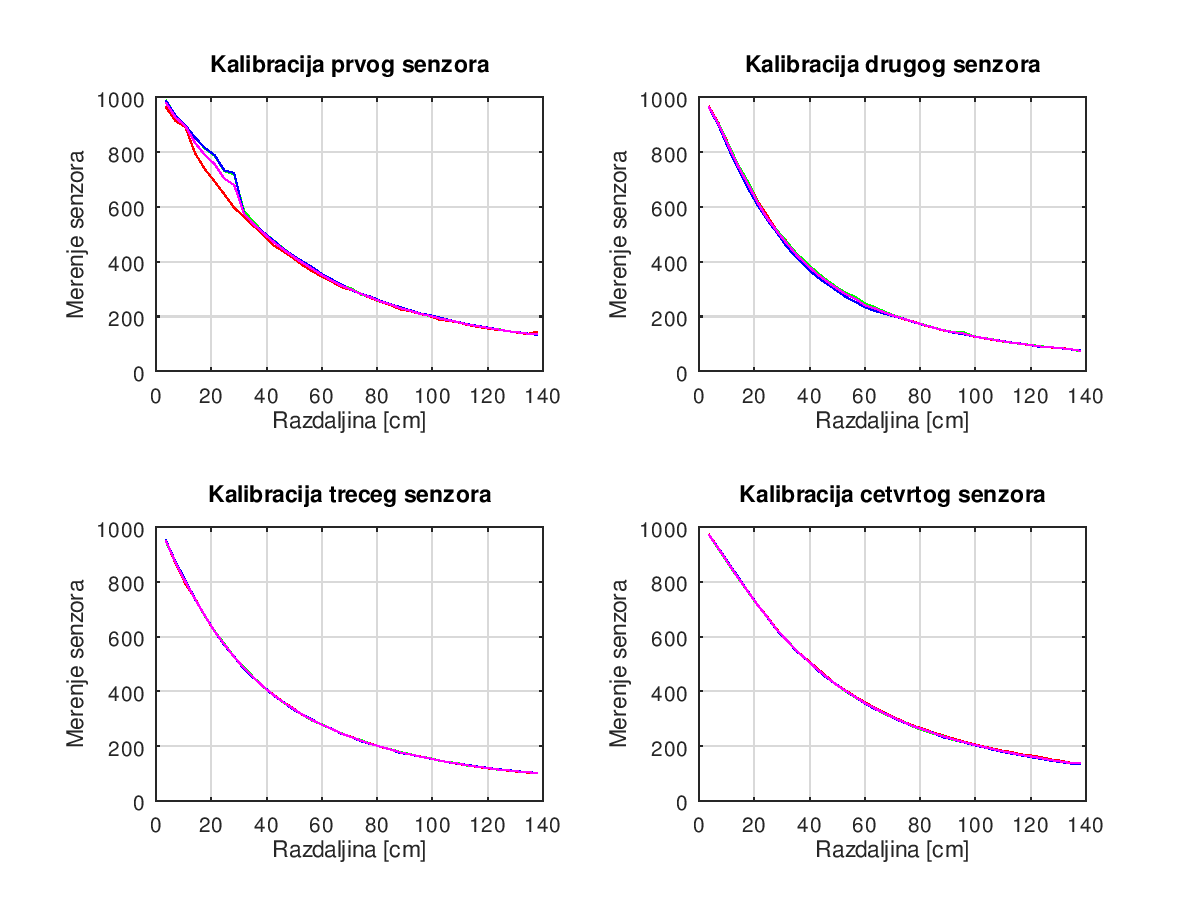
\includegraphics[scale=0.6]{kalibracija.png}
        \caption{Grafici zavisnosti izmerenih udela napona od razdaljine senzora. Može se primetiti da je zavisnost kvadratna funkcija, pa je stoga na sledećem koraku vršena linearizacija.}
        \label{Kalibracija}
    \end{figure}

    Nakon merenja izvršena je linearizacija funkcije zavisnosti napona od udaljenosti (dobijena funkcija je bila funkcija zavisnosti recipročne vrednosti kvadratnog korena napona od udaljenosti) i njena aproksimacija metodom najmanjih kvadrata uz pomoć \textit{MATLAB}-a. Takođe je vršena aproksimacija greške. % koja to beše greška maksimalna ili prosečna? [Možda objasniti metodu najmanjih kvadrata u finalnoj verziji]

    Na osnovu aproksimiranih funkcija iz kalibracije mogla je za svaku izmerenu vrednost senzora mogla da bude određena razdaljina objekta od senzora, tako da je sledeći korak bio saznavanje lokacije objekta u dvodimenzionalnom prostoru (stolu) na osnovu razdaljine izmerene sa tri senzora. To je urađeno korišćenjem trilateracije, metodom povlačenja tri kružnice iz tri senzora poluprečnika dužine izmerene razdaljine i pronalaženje centra njihovog preseka (odnosno tačke najmanje udaljene od sve tri kružnice u slučaju da se kružnice ne seku).

    Nakon rešavanja pomenutih problema, pređeno je na izradu programa i elektronskih kola za vizuelizaciju lokalizacije. To je realizovano tako što je svaki senzor bio povezan na naponske razdelnike u kojima su $R_1$ otpornici jačine \SI{1}{\kilo\ohm} a $R_2$ otpori sa fotootpornika. Izlazni napon povezan je na analogne pinove na \textit{EasyPIC}-u sa kojih je čitano u mikroC programu koji je te podatke slao na UART. Sa UART-a je čitao \textit{Progressing} program koji je na osnovu udela napona određivao razdaljinu objekta od senzora, vršio trilateraciju da bi odredio poziciju objekta na tabli i onda tu poziciju iscrtavao na ekranu zajedno sa kružnicama oko senzora koje su korišćene pri trilateraciji. Tokom vežbe nije vršena "prava" trilateracija, već je program za $100\times100$ tačaka table određivao razliku između udaljenosti od senzora i izmerene udaljenosti od senzora i postavljao poziciju objekta na tačku s najmanjom razlikom.

    Naknadno je dodat i modul koji je omogućavao dalje smanjivanje rezolucije, tako da su omogućena merenja do 0.5cm. Sam modul je bio kvadratnog oblika i postavljao se preko 4 tačke na stolu. Modul je imao 6x6 rupica.

    \begin{figure}[H]
        \subfloat[]{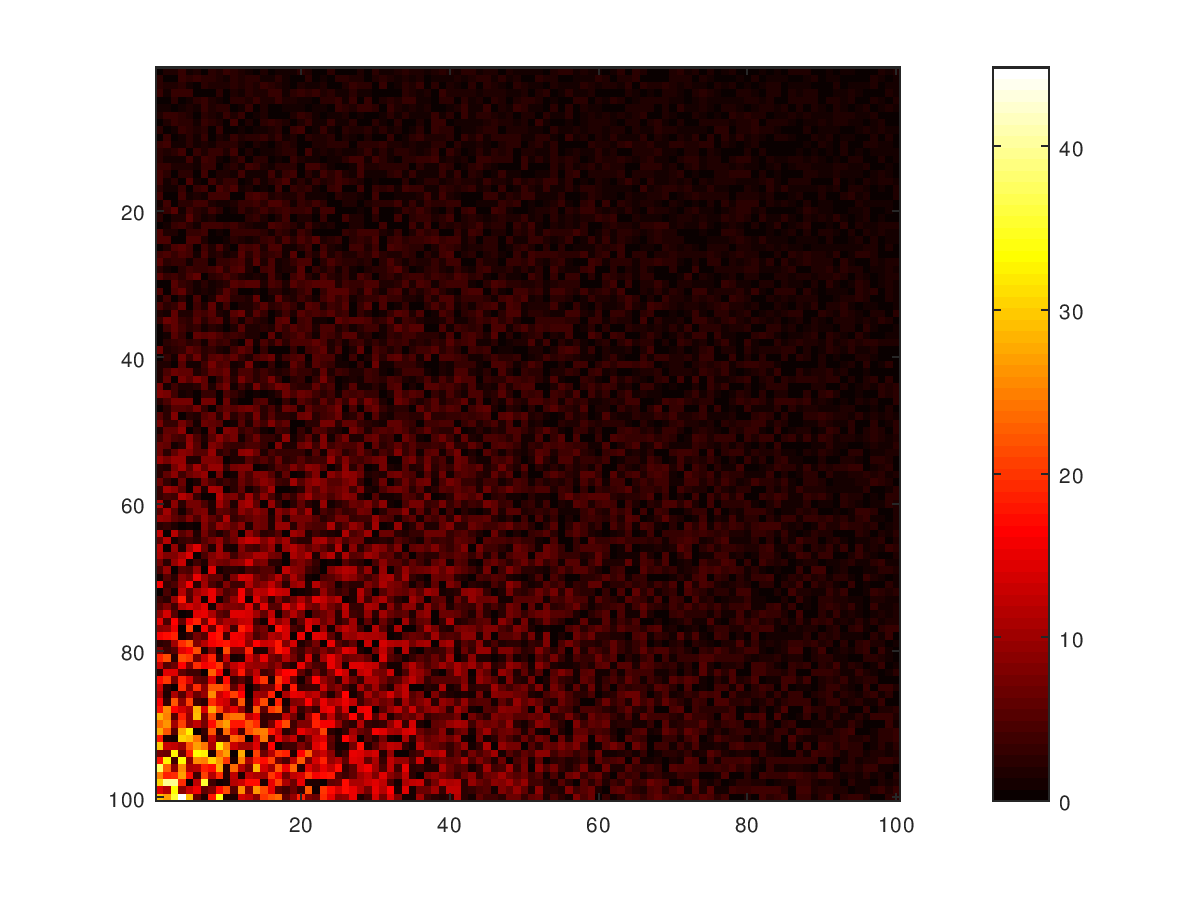
\includegraphics[scale=0.2]{greska-1.png}}
        \subfloat[]{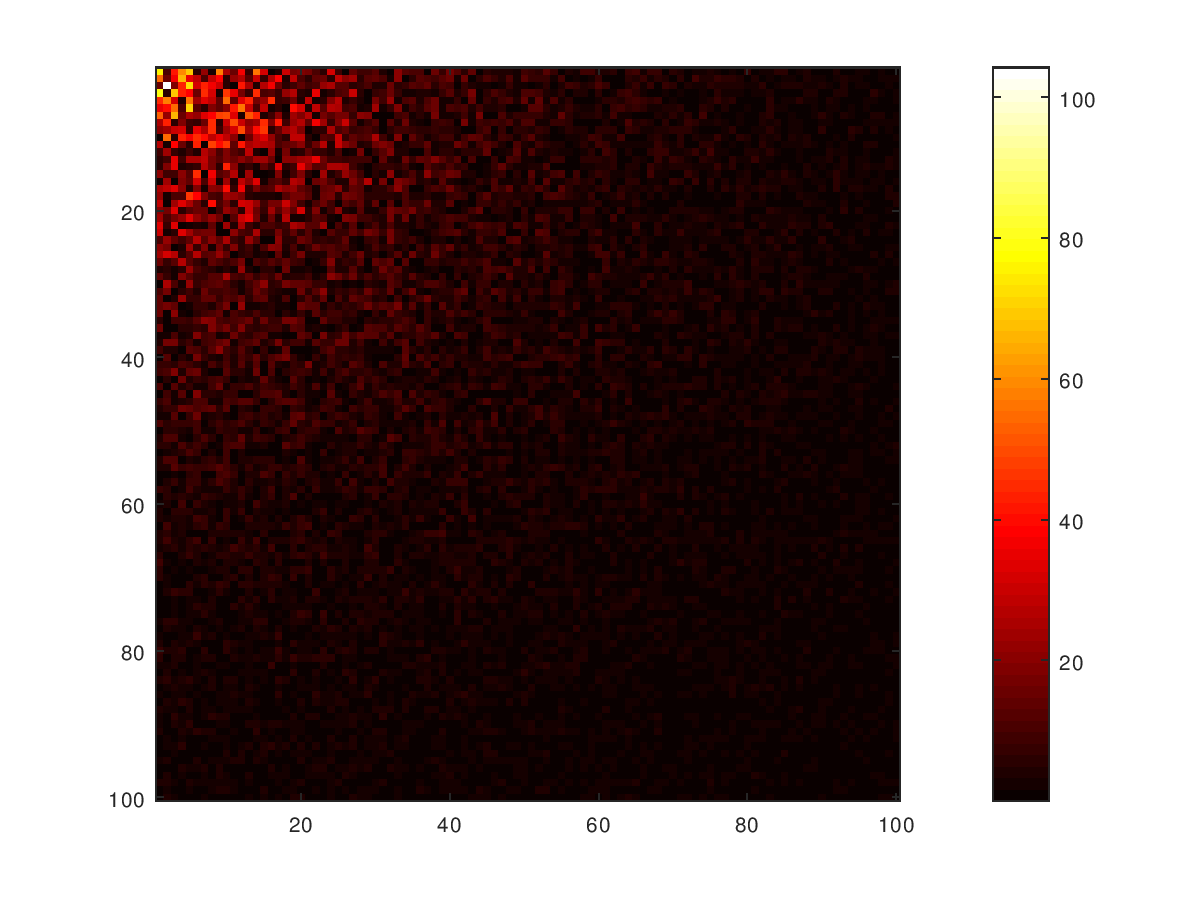
\includegraphics[scale=0.2]{greska-2.png}}
        \subfloat[]{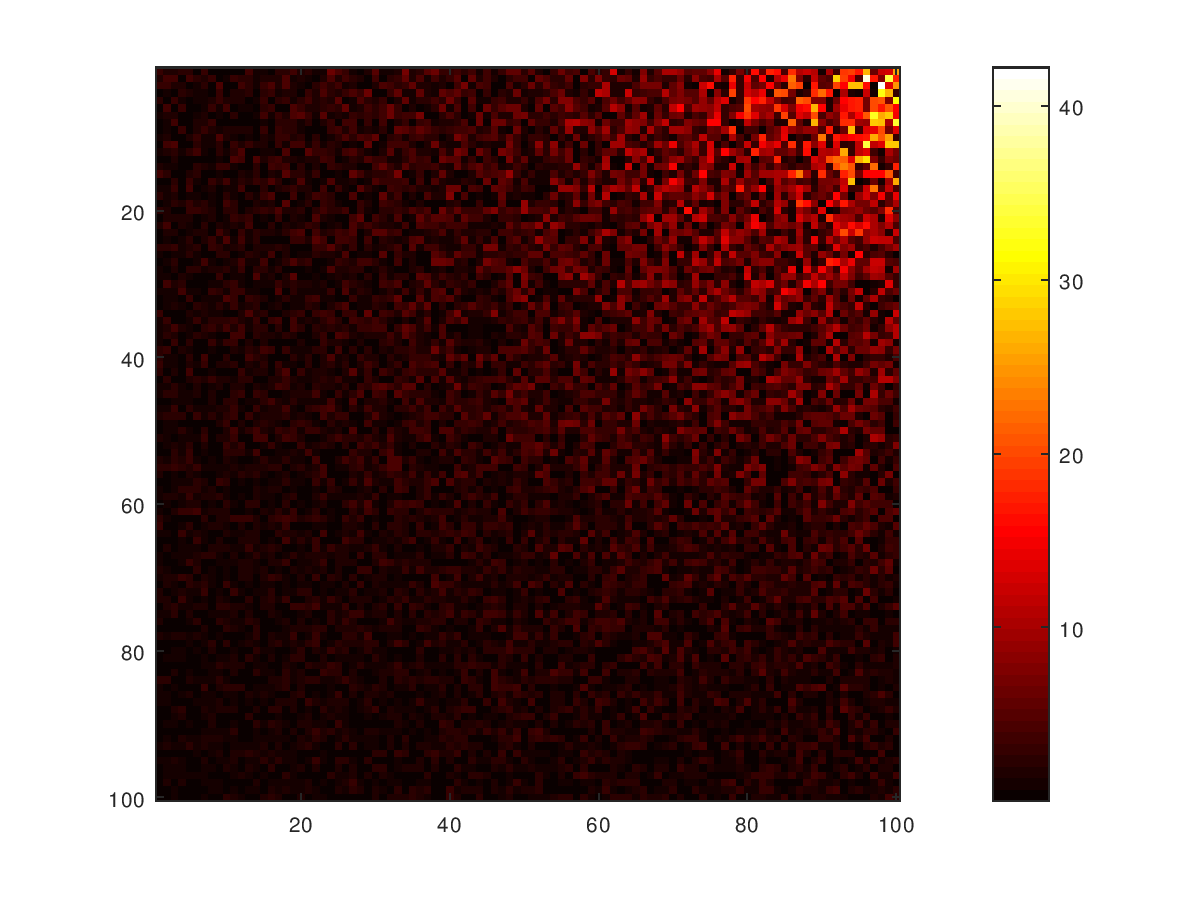
\includegraphics[scale=0.2]{greska-3.png}}
        \caption{\textit{Heatmap}-e izmerenih greški u simulaciji}
        \label{Greska}
    \end{figure}

    U \textit{Processing}-u je takođe napravljena simulacija radi upoređivanja realnih merenja sa idealnim. U simulaciji su senzori bili idealni, te se pozicija sijalice nije morala računati ranije korišćenom "Brute Force" metodom nego je moguće poziciju sijalice izračunati formulom:
    $$y_1 = \sqrt{r_2^{2}-x_1^{2}}$$
    $$x_1 = \sqrt{r_2^{2}-y_1^{2}}$$
    $$y_1 = \sqrt{r_1^{2}-(x-x_1)^{2}}$$
    $$x_1 = \sqrt{r_3^{2}-(y-y_1)^{2}}$$
    \newline
    sledi, 
    $$r_3^{2}-(y-y_1)^{2} = r_2^{2}-y_1^{2}$$
    $$r_3^{2}-y^{2}+2yy_1 = t_2^{2}-y_1^{2}$$
    $$r_3^{2}-y^{2}+2yy_1 = r_2^{2}$$
    $$2yy_1 = r_2^{2}+y^{2}-r_3^{2}$$
    $$y_1 = \frac{r_2^{2}+y^{2}-r_3^{2}}{2y}$$
    gde je:
    \begin{itemize}
        \item $r_1$ - rastojanje sijalice od senzora 1
        \item $r_2$ - rastojanje sijalice od senzora 2
        \item $r_3$ - rastojanje sijalice od senzora 3 (nasuprot senzoru 1)
        \item $y$ - poznata dužina mernog područja
        \item $x$ - poznata širina mernog područja
        \item $y_1$ - tražena y koordinata sijalice
        \item $x_1$ - tražena x koordinata sijalice
    \end{itemize}
    Slično se izvodi i formula za $x_1$. Dobijena merenja iz simulacije su zatim ubačena u Octave, i napravljene su \textit{heatmap}-e grešaka senzora. Kao što se može videti sa slike \ref{Greska}, najveće izmerene greške mogu se videti u područjima oko senzora.

    \begin{figure}[H]
        \centering
        \subfloat[]{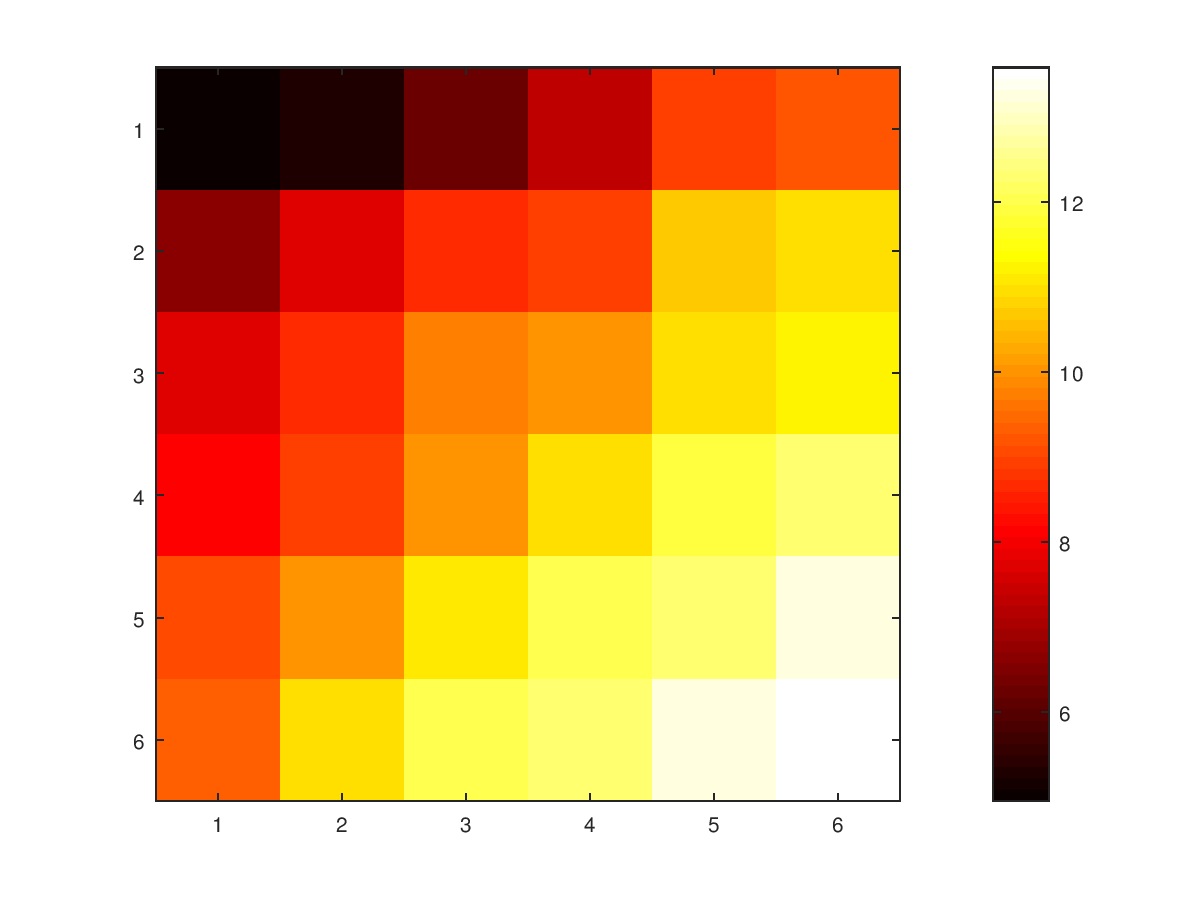
\includegraphics[width=0.475\textwidth]{nw.png}}
        \subfloat[]{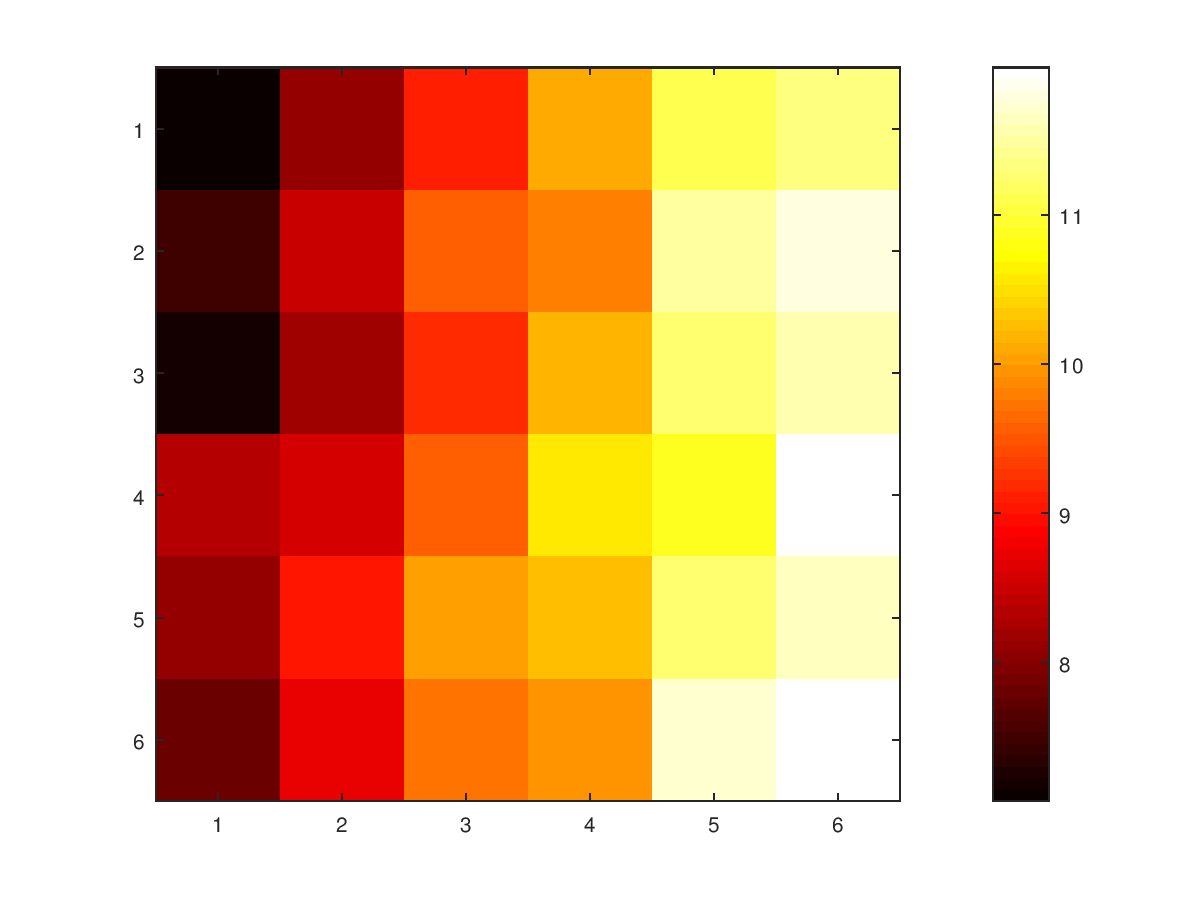
\includegraphics[width=0.475\textwidth]{ne.png}} \\

        \subfloat[]{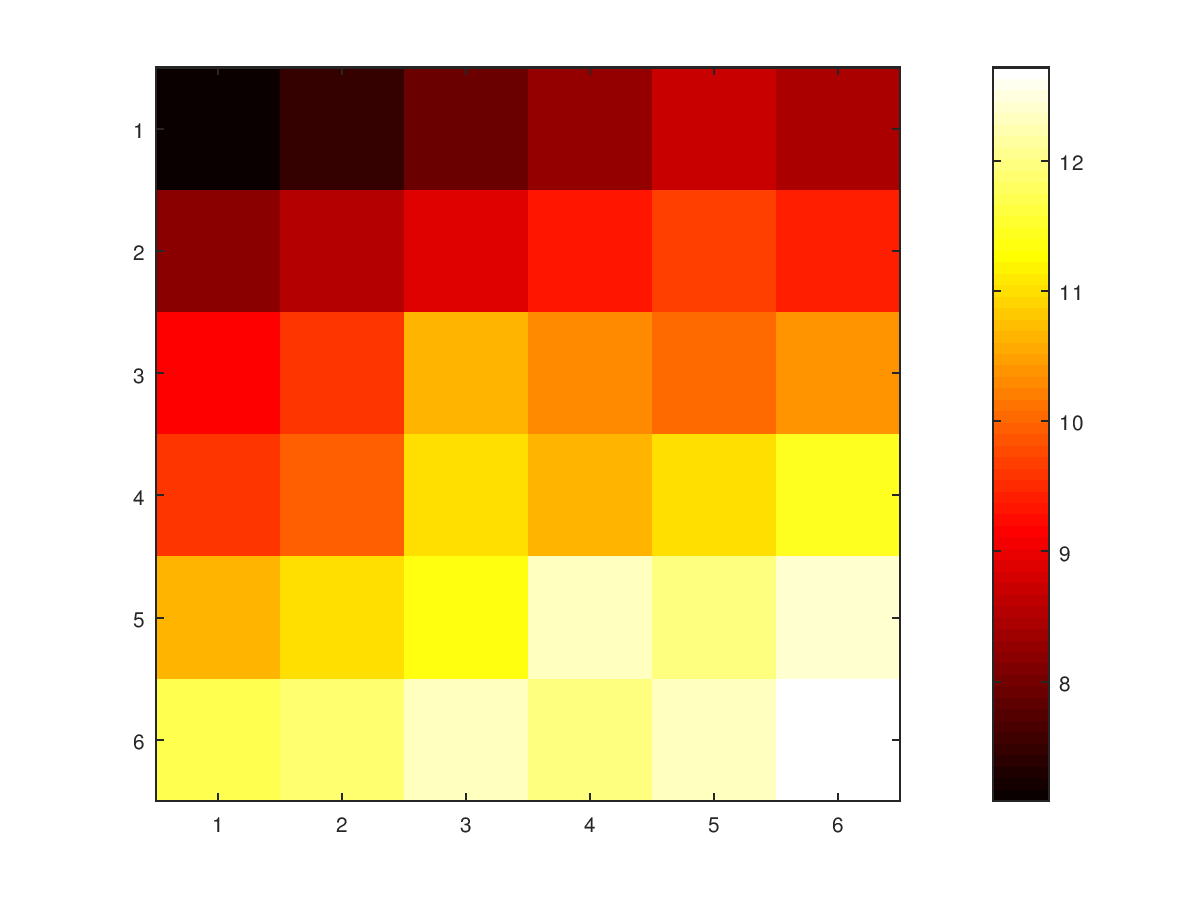
\includegraphics[width=0.475\textwidth]{sw.png}}
        \subfloat[]{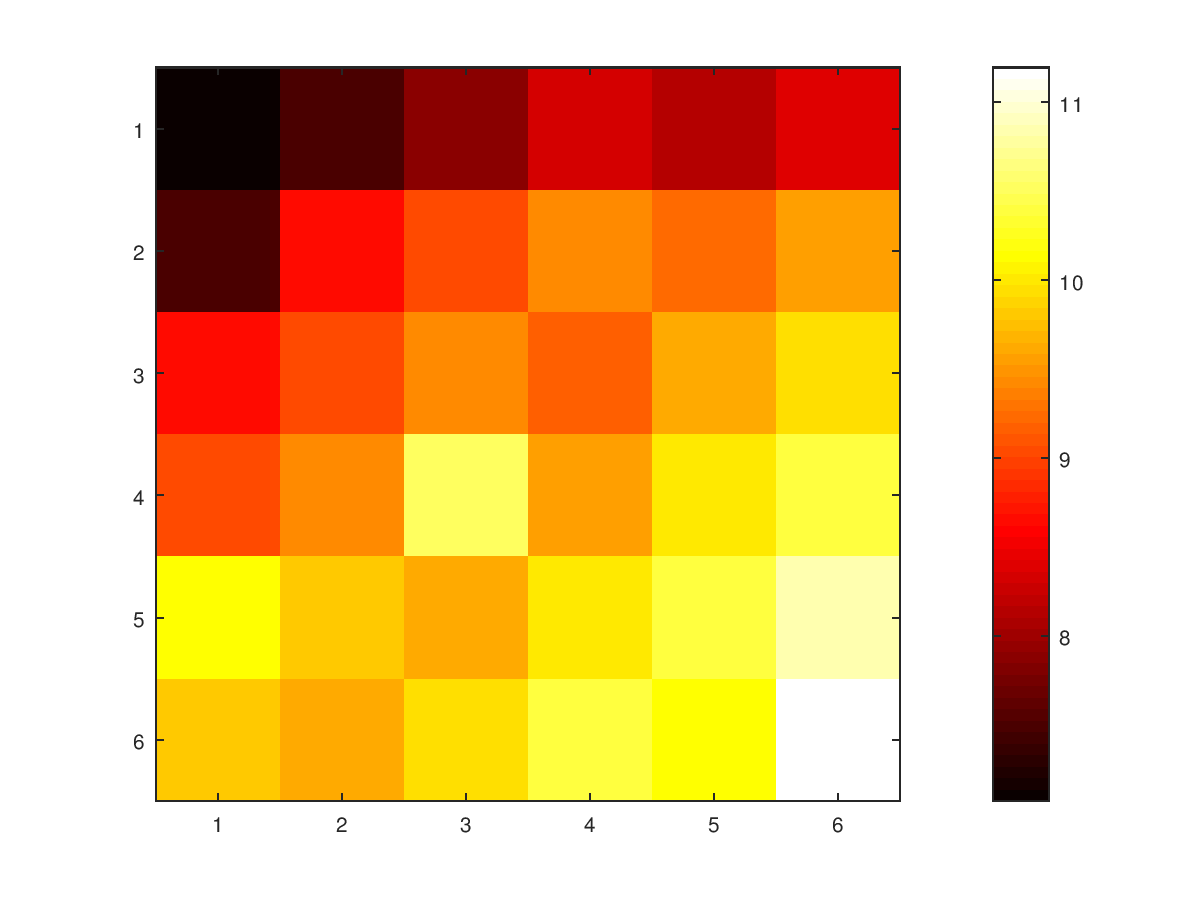
\includegraphics[width=0.475\textwidth]{se.png}}
        \caption{Merenja greške programa po centru table, svako merenje je udaljeno \SI{0.5}{\cm}}
        \label{Centar}
    \end{figure}

\section{Zaključci i rezultati}
    Najveća greška u merenju bila je \SI{1.82}{\cm}, a najmanja greška \SI{0.01}{\cm}. Zaključeno je da su merenja najtačnija u samom centru mernog područja, gde sistem meri sa greškom manjom od \SI{0.7}{\cm}. Merenja su najnetačnija na ivicama table, gde je sistem merio sa greškom od oko \SI{3.2}{\cm}. To se dešava zbog neidealnosti senzora.

    Uz pomoć gorepomenutog \textit{Processing} programa, zabeležene su lokacije koje su dobijene nakon trilateracije Monte Karlovim metodom za svaku od 1681 tačaka table. Uz pomoć \textit{Octave}-a, na osnovu izmerenih lokacija određena je greška programa i predstavljena kao još jedna \textit{heatmap}-a koja se može videti na slici \ref{Merenje}.

    %Trilateracija Monte Karlovim metodom podrazumeva % ...

    Iako nije bilo potrebno, osposobljen je i kalibrisan četvrti senzor. Izvršena merenja sa četvrtim senzorom uključenim pokazivala su dosta tačnije rezultate, pogotovo na području oko četvrtog senzora. Razlika prosečne greške sistema sa 3 senzora i sistema sa 4 senzora je \SI{0.52}{\cm}.

    \begin{figure}[H]
        \centering
        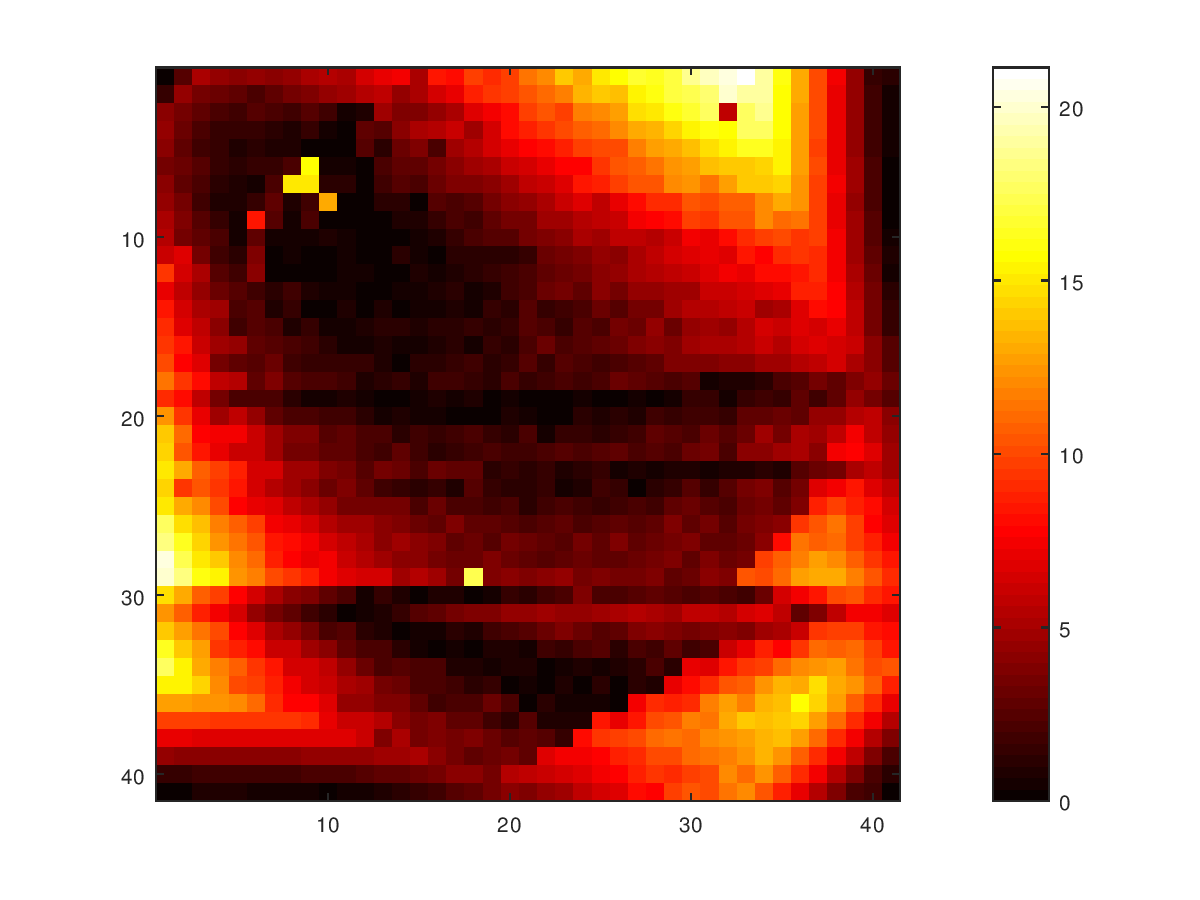
\includegraphics[scale=0.3]{merenje.png}
        \caption{Greška određivanja lokacije programa po celoj tabli}
        \label{Merenje}
    \end{figure}

\section{Literatura}
    \begin{itemize}
        \item GNU Octave Documentation, (2018). \textit{Representing Images}. [online] Available at: \url{https://octave.org/doc/v4.2.2/Representing-Images.html#index-colormap}, [Pristupljeno: 22.09.2018. g.]
        \item Resistor Guide, (2018). \textit{Photo resistor - Light Dependent Resistor (LDR)}. [online] Dostupno na: \url{http://www.resistorguide.com/photoresistor/}, [Pristupljeno: 22.09.2018. g.]
        \item Processing, (2018). \textit{Language Reference (API)}. [online] Dostupno na: \url{https://processing.org/reference/}, [Pristupljeno: 22.09.2018. g.]
    \end{itemize}
\end{document}
